\chapter{Symbolic Cross-References\label{chap:blah}}

This chapter has more information on symbolic cross-referencing.
In addition, there are examples showing how to typeset a figure
and a simple table.

\section{Figures}

Figure~\ref{fig:encrypted_virus} has been typeset so that it
occupies half the width of text on a page ({\tt width=0.5}). Note the 
symbolic cross-reference, that is, you simple \verb+\ref{fig:encrypted_virus}+
to obtain the appropriate number for Figure~\ref{fig:encrypted_virus}.

\begin{figure}[htb]
\centering
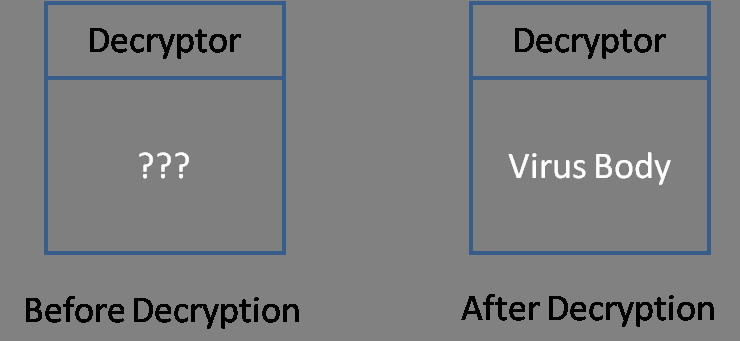
\includegraphics[width=0.5\textwidth]{images/encrypted_virus.jpg}
\caption{Encrypted virus before and after decryption.} 
\label{fig:encrypted_virus}
\end{figure}

If you move things around, insert or delete text, Figure~\ref{fig:encrypted_virus}
will still give you the correct number. This is a very handy feature.


\section{Tables}

Table~\ref{tab:19} 
shows some interesting stuff. I hope you enjoy it.

\begin{table}[htb]
\caption{MysteryTwister Zodiac Challenge\label{tab:19}}
\begin{center}
\begin{tabular}{c|lc}\hline\hline
Case & \multicolumn{1}{c}{Description} & Percentage\\ \hline
1F & Fast outer hill climb and English stats & 13.00\% \\
1S & Slow outer hill climb and English stats & \phantom{0}4.00\% \\
2F & Fast outer hill climb and Zodiac~408 stats & 70.00\% \\
2S & Slow outer hill climb and Zodiac~408 stats & 84.00\% \\ \hline\hline
\end{tabular}
\end{center}
\end{table}


\section{Citations}

References are cited using the \verb+\cite+ command. For example,
see~\cite{harden} for information on the Zodiac killer. You can include more than one 
reference in a single citation, like this~\cite{harden,bib1,basa,bib3,bib2,glurk,bib7,bib10,bib11}
or this~\cite{bibAC,bib17}.


\section{The Last Word}

There are a lot of other uses for symbolic cross-referencing. For example, this chapter
title has a label so I can refer to Chapter~\ref{chap:blah} (as I just did).
My recommendation is that you include a label with anything and everything that 
is numbered. If it has a number, there is a good chance that you will
refer to it at some point.

Finally, note that you need to \LaTeX\ a file at least twice (three times to
be safe) without changing anything to be sure that the numbering is correct.
Why is that? Good question.
When you \LaTeX\ your document, various auxiliary files are created. Most of these files contain
information related to cross-references that appear in your {\tt .tex} file (or files). The next time you 
\LaTeX\ your document, the information from the previous run is read from
these auxiliary files. Consequently, after making changes to any {\tt .tex}
file, you will need to \LaTeX\ your document at least twice to be sure that the
cross-reference information is updated in the resulting pdf. In fact, you should
run \LaTeX\ three consecutive times to be certain that cross-references are correct.

